\documentclass[preprint,12pt]{elsarticle}


\usepackage[spanish]{babel}
\usepackage{amssymb}
\usepackage{graphicx}
\usepackage{lineno}
\usepackage[utf8]{inputenc}
\usepackage{url}
\usepackage{cite} 




\journal{Data Story Telling}

\begin{document}
	\begin{frontmatter}
		
		
		\title{\huge Data Story Telling}
		
		
		\author{Escalante Maron, Nelia (2014049551)  
			\\Condori Gutierrez, Flor (2015053227)
			\\Coaquira Calizaya, Yerson (2015053225)
			\\Cespedes Medina, Christian (2010036256)   
			\\Arteaga Ramos, Javier Octavio (2007028981)  }
		
		\address{Tacna, Peru}
		
				
		\begin{abstract}
			
			%% Text of abstract
			El mundo de la visualización de datos es fascinante, pero el éxito de una buena visualización no solo radica en el análisis y creación de gráficas con datos sino más bien en la organización de la información y la narrativa de los mismos. 
			El data storytelling, tal como lo señala GlobalWebIndex, se trata de generar conexiones usando datos como la fuente que guíe a la marca. Ya sea que se emplee para dar forma a una identidad de marca única o para generar una campaña de marketing de impacto, el data storytelling aporta a las marcas la oportunidad de capturar la atención de una forma que se centra enteramente en la audiencia objetivo. Las historias que están formadas de esta forma son las que logran darles vida a las marcas.\\
			
			\textit{The world of data visualization is fascinating, but the success of a good visualization not only lies in the analysis and creation of graphs with data but rather in the organization of the information and the narrative thereof.
			Data storytelling, as GlobalWebIndex points out, is about generating connections using data as the source that guides the brand. Whether used to shape a unique brand identity or to generate an impact marketing campaign, data storytelling gives brands the opportunity to capture attention in a way that focuses entirely on the target audience. The stories that are formed in this way are those that manage to give life to the brands.}
						
		\end{abstract}
		
	\end{frontmatter}
	%%
	%% Start line numbering here if you want
	%%
	%\linenumbers
	
	%% main text
	\newpage
	\section{INTRODUCCION}
	\label{S:1}
	El Data Storytelling es una herramienta que emplea la combinación de datos estadísticos y comunicación. Ayuda a las empresas a cumplir metas de comunicación y marketing contando mensajes de manera efectiva y cargados de información relevante para el público objetivo, también apoyados en instrumentos visuales y narrativos.\\
	\\
	Para poder llevar a cabo la implementación del Data Storytelling, es necesario contar con algunas herramientas de tecnologías de la información, tales como: base de datos que nos permitirá comprender el comportamiento y contextos de los grupos a los que queremos dirigirnos, buscaremos datos que nos permitan generar un insight en común, esta base de datos se puede enriquecer, a través de encuestas o formularios brindados por los grupos de interés, es indispensable contar con computadoras y tablets que apoyen la elaboración del contenido a presentar.\\
	\\
	Se pueden emplear las diferentes redes sociales para difundir las historias con los respectivos mensajes que queremos hacer llegar a nuestros grupos objetivos, es por esto que también es necesario poder conocer los máximos beneficios que éstas pueden ofrecer, ya que de nada serviría enviar los mensajes a personas que no formen parte del grupo al que queremos llegar.
	
	\section{OBJETIVOS}
		\begin{enumerate}[a)]
			\item Las historias son herramientas efectivas para transmitir la experiencia humana: esto ha sido así desde el inicio de los tiempos, pero ahora utilizamos datos y análisis para crear versiones mejoradas de esas historias. Gracias a ellas simplificamos y damos sentido a un mundo complejo.
			\\
			\item Para inspirar el cambio, necesitamos que entiendan nuestra historia: no importa cuántas horas hay detrás de nuestro análisis, no lograremos nada si no nos logramos explicar ya sea con una narrativa o con gráficos pero, necesitamos una historia.
			\\
			\item Las personas quieren evidencia del análisis que hay detrás: aunque nuestra audiencia no entienda el detalle de la analítica, sí quieren la evidencia de que hay datos detrás, ya que estas historias son más convincentes que solo una experiencia personal.
			\\
			\item Contar en una breve historia el resultado de horas de trabajo: se necesitan presentaciones cortas, con ideas concretas adaptadas a los stakeholders que recibirán la información para hacer llegar tu mensaje de una manera simple. 
		\end{enumerate}
	
	\section{MARCO TEÓRICO}
	\textbf{ STORY TELLING}\\
	
	Philippe Nieuwbourg: “El Storytelling es el arte y la manera de contar una historia dándoles un toque humano y el Data Storytelling es el arte y la manera de contar una historia apoyándose en los datos, cifras, o hechos, ya que si tomamos una gráfica o una simple curva ésta no cuenta ninguna historia. Entonces, el Data Storytelling ayuda a crear una historia que permitirá explicar las cifras y los datos”. \\
	\\
	Por ponerlo de una forma más simple, la firma Analítica Web señala que el llamado data storytelling no es más que un enfoque estructurado sobre cómo se comunican insights a partir de datos, este enfoque se vale de datos, visualización y narrativa, y la combinación de estos elementos deriva en distintos resultados, por ejemplo, la suma de la narrativa y los datos permite “explicar”, la suma de la visualización y los datos, permite “ilustrar”, y la suma de la narrativa con la visualización aporta como resultado el “entretenimiento”. La suma de los tres elementos arroja como resultado un el concepto de “cambio”. [\citen{bib01}]\\

\textbf{ELEMENTOS CLAVE DEL DATA STORYTELLING}\\
	
	El llamado Data Storytelling no es más que un enfoque estructurado sobre cómo comunicamos insights a partir de los datos, e involucra una combinación de tres elementos: 
	\begin{itemize}
		\item Ciencia de los Datos o datos
			
		Tal como lo destacamos hace poco la data science o ciencia de datos consiste en la práctica de revelar insights ocultos en los datos existentes aun una forma que habilite a las empresas a tomar mejores decisiones se trata de un concepto que puede ayudar a mejorar el rendimiento y crecimiento de un negocio.
		
		
		\item Visualizaciones
		
		Transformar data en gráficos, tablas o formatos similares significa que se puede visualizar la data como una antes. Las visualizaciones ahora son posibles y mejores gracias a las soluciones de tecnologías emergentes que nos ayudan a comprender cantidades importantes de información recolectada.  Las visualizaciones de datos por sí solas tienen limitaciones, por ello, el tercer campo de exprese es la narrativa.
		
		\item Narrativa
		
		Dentro del data storytelling, la narrativa se puede considerar el elemento más importante. La narrativa utiliza el lenguaje en un formato que se adecua a ciertas necesidades en particular aumentando la comprensión de nueva información, es el vehículo clave para transmitir insights.\\
		\\
		Resultado de las uniones de los elementos:
		
		\begin{center}
			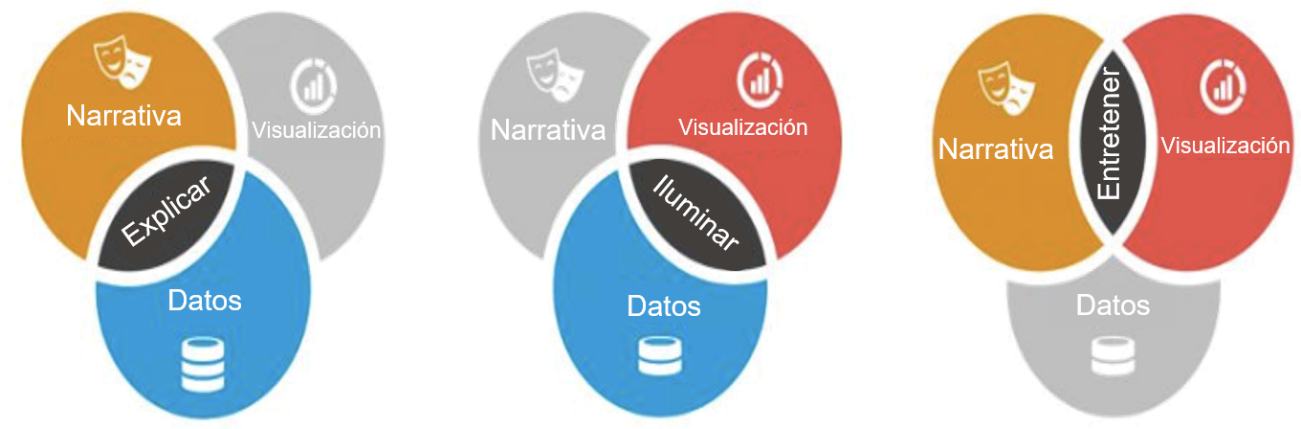
\includegraphics[width=13cm]{./Imagenes/img1} 
		\end{center}
		
			\begin{itemize}
				\item Narrativa + Datos = Explicar. Podremos explicar qué ha pasado y por qué un insight puede ser importante. Necesitaremos contexto para entender las conclusiones por completo.
				\item Visualización + Datos = Iluminar. Cuando añadimos una visualización a nuestros datos, podemos iluminar a nuestra audiencia con insights que no habrían visto de otra manera.
				\item Narrativa + Visualización = Entretener. La combinación perfecta para lograr ese interés e incluso para entretener a nuestra audiencia.
			\end{itemize}

	\end{itemize}
	Cuando se reúne la Visualización + Narración + Datos = Cambio, se logra contar una historia con datos, se logra influenciar y llevar a ese cambio que se está buscando [\citen{bib02}].
	
	\begin{center}
		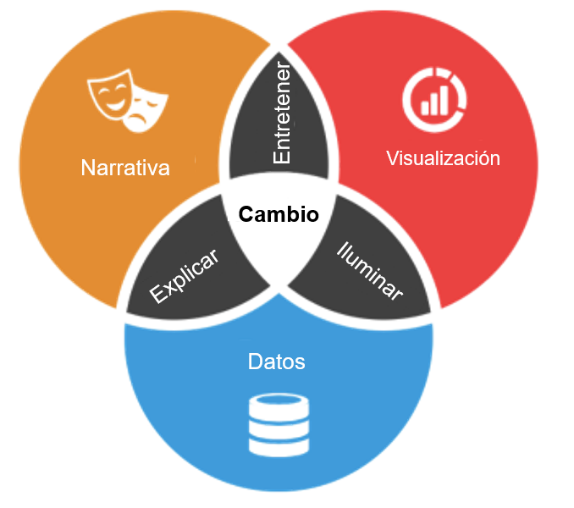
\includegraphics[width=7cm]{./Imagenes/img2} 
	\end{center}

	\section{IMPORTANCIA}
	
	Contar una gran historia basada en datos puede ser útil tanto para las partes interesadas como para sus clientes y puede impulsar una mejor toma de decisiones dentro de una organización y también impulsar conversiones con sus clientes. Al utilizar la visualización de datos para hacer observaciones clave sobre sus clientes y sus necesidades, puede ayudar a generar clientes potenciales y retener clientes.\\
	\\
	Algunas de las razones por las que es importante emplear esta herramienta dentro de una organización, o de manera personal, son las siguientes:
	
	\begin{itemize}
		\item En primer lugar, la importancia radica en la riqueza de la información con la que se cuenta dentro de una base de datos y el aporte que ésta brinda al momento de contar una historia.
		\item También permite simplificar toda la información que las organizaciones quieren transmitir a sus diferentes grupos de interés, ya sean clientes, colaboradores, proveedores, accionistas.
		\item Finalmente, permite representar de manera más sencilla y dinámica el mensaje. Empleando la narrativa, logramos que el mensaje sea interpretado de la manera en que deseamos.
	\end{itemize}
	\textbf{VENTAJAS DEL DATA STORYTELLING}\\
	
	Retomando la información publicada por Analítica Web, el concepto de data storytelling cuenta con al menos 4 ventajas considerables, estas son: 
	
	\begin{enumerate}[A.)]
		\item Comprensión rápida de la información
		Debido a que el data storytelling puede mejorar la visualización de la información, podemos ser capaces de ver grandes cantidades de datos de forma clara y coherente, aspecto que facilita la obtención de insights y la generación de conclusiones.
		\\
		\item Identificación para actuar rápido sobre las tendencias emergentes
		Con el data storytelling es posible comprender archivos de datos muy amplios cuando son representados gráficamente, ello permite detectar parámetros correlacionados.
		\\
		\item Identificación de relaciones y patrones dentro de los activos digitales
		Tal como lo destaca desde su sitio, el descubrir tendencias dentro de los datos, permite una ventaja competitiva importante, la de detectar puntos clave que están afectando a elementos como la calidad del producto, o bien, solucionar incidentes antes de que estos lleguen a un mayor grado.
		\\
		\item Desarrollo de un nuevo lenguaje de negocio para contar la historia a terceros
		Finalmente, destaca que gracias al data storytelling es más fácil transmitir los mensajes y lograr impulsar el entretenimiento.
		
	\end{enumerate}
	
	\textbf{PROCESO DE EJECUCION E IMPLEMENTACION DEL DATA STORYTELLING}\\
	
	A continuación, se explica cómo se debería realizar el proceso de ejecución e implementación del Data Storytelling:
	
	\begin{itemize}
		\item El primer paso es el reconocimiento del público al cual se dirigirá el Data Storytelling.
		\item Luego, necesitamos encontrar un insight para generar contenido relevante.
		\item Paso siguiente, crear contenido para aplicar el insight encontrado con la información que se busca transmitir.
		\item Posteriormente, comunicar el contenido elaborado al público objetivo.
		\item Después, se tiene que mantener el Data Storytelling.
		\item Por último, se debe realizar una evaluación del Data Storytelling.
	\end{itemize}
	Para poder llevar a cabo la implementación del Data Storytelling, es necesario contar con algunas herramientas de tecnologías de la información, tales como: base de datos que nos permitirá comprender el comportamiento y contextos de los grupos a los que queremos dirigirnos, buscaremos datos que nos permitan generar un insight en común, esta base de datos se puede enriquecer, a través de encuestas o formularios brindados por los grupos de interés, es indispensable contar con computadoras y tablets que apoyen la elaboración del contenido a presentar.\\
	\\
	\textbf{ERRORES AL EMPLEAR EL DATA STORY TELLING}\\
	
	Las personas analíticas a menudo no son tan motivadas o exitosas para comunicarse con formas de vida basadas en el carbono. Gravitaron hacia campos estructurados, no ambiguos e invariables, como matemáticas, estadística y ciencias de la computación en la escuela, y continúan favoreciendo la interacción con números sobre la interacción con humanos en sus carreras laborales. Por supuesto, no todos los analistas cuantitativos son de esta persuasión, y alguien con un fuerte enfoque numérico puede hacer una transición en el tiempo para ser más humano y literario en sus orientaciones. Pero reconozcamos que contar historias convincentes a otros humanos puede no ser algo natural para muchos analistas.\\
	\\
	Si los analistas no se inclinan naturalmente hacia la narración de cuentos, probablemente tampoco reciban mucha instrucción al respecto en la escuela. Muchos profesores universitarios que imparten cursos cuantitativos no son en sí mismos terriblemente buenos para contar historias. Y pueden sentir que es más importante impartir más instrucción sobre los métodos que "perder el tiempo" en los enfoques de narración.\\
	\\
	Para dedicarse a la narración, algunos analistas pueden creer que es un insulto, o al menos una inversión de tiempo relativamente menos valiosa en comparación, con las capacidades técnicas de un analista. Los analistas cuantitativos capaces pueden argumentar justificadamente que muchas personas pueden contar buenas historias, pero relativamente pocas pueden ejecutar un modelo de regresión logística con correcciones de heterocedasticidad. Pueden sentir que el mejor uso de su tiempo y las células cerebrales es hacer un análisis cuantitativo y confiar en que otros cuenten historias al respecto. Pueden tener un punto, pero confiar en otros para traducir los resultados analíticos en historias tiene sus propios peligros, además de ser más laborioso.\\
	\\
	A los analistas les lleva mucho tiempo pensar creativamente sobre cómo contar una buena historia con datos. De hecho, un analista senior de una compañía farmacéutica me dijo que él (y la mayoría de los miembros de su grupo de análisis) pasan la mitad de su tiempo pensando en la mejor manera de comunicar sus resultados analíticos. Muchos analistas estarán renuentes a dedicar tanto tiempo al tema, incluso si eso los hiciera más efectivos. [\citen{bib04}]\\
	\\
	\textbf{CÓMO REALIZAR UN CORRECTO DATA STORYTELLING}
	
	\begin{center}
		
\includegraphics[width=10cm]{./Imagenes/img3} 
	\end{center}

	La narración de datos puede parecer intimidante, y para aquellos que provienen de una formación decididamente no matemática, puede parecer una lengua extranjera. Pero los especialistas en marketing pueden ser realmente más eficaces para dar vida a historias de datos.
	Los analistas y estadísticos tienen habilidades técnicas fantásticas, pero cuando se trata del elemento humano, a menudo les resulta difícil traducir de manera efectiva todos esos puntos de datos en una historia interesante.\\
	\\
	Los profesionales de marketing saben a quién están tratando de llegar, por lo que es más fácil traducir esos datos a un idioma que entiendan. Si te sumerges en la narración de datos, hay ciertos elementos que garantizarán que tenga éxito.
	
	\begin{enumerate}[A)]
		\item Elegir el tema correcto
		
		La gran narración de datos necesita una historia interesante. Si bien los datos pueden dar un giro interesante a un tema aburrido, asegúrese de que sea algo relevante o interesante para las personas a las que intenta llegar. Tenga en cuenta que la narración de datos no es una historia sobre números; Se trata de cómo esos números afectan a los humanos.\\
		\\
		A veces, es posible que tenga una idea de la historia y necesite evaluar los datos para ver si tiene patas. En otras ocasiones, es posible que encuentre una gran información en un conjunto de datos sólidos y construya su historia a partir de ahí.\\
		
		\item Fuentes de datos creíbles
		
		La narración de datos genera confianza, pero solo cuando se basa en datos sólidos. Los datos se pueden manipular, tergiversar o malinterpretar fácilmente, por lo que tener una fuente sólida y sin sesgos es increíblemente importante.\\
		
		\item Elabore una narrativa interesante, interesante y esclarecedora
		
		La buena información sola no hace una buena historia de datos. La narración de datos solo es efectiva cuando proporciona valor, ya sea que enseñe algo nuevo a las personas, les brinde una nueva perspectiva o los inspire a tomar medidas.\\
		\\
		La forma en que usted entrega esa historia determina si ese mensaje se comunica. Su narrativa debe guiar a los lectores, proporcionarles un contexto y ayudarlos a sintetizar la historia de los datos de la manera más efectiva posible.\\
		
		\item Datos de diseño según las mejores prácticas
		
		Una de las mejores maneras de sabotear su narración de datos es con visualizaciones de datos incorrectamente o mal diseñadas. La visualización de datos está diseñada para hacer que los datos sean lo más fáciles de entender posible, por lo que es importante trabajar con un diseñador que entienda las mejores prácticas.
		
	\end{enumerate}
	
	Esto conlleva a:
	\begin{itemize}
		\item \textbf{Comprensión rápida de la información:} gracias a las representaciones gráficas podemos ver grandes cantidades de datos de forma clara y coherente, lo que facilita la extracción de conclusiones e insights. Ganaremos tiempo y eficiencia para solucionar problemas.
		\item \textbf{Identificar y actuar rápido sobre tendencias emergentes:} incluso los archivos de datos casi infinitos, empiezan a tener sentido al representarse gráficamente; lo que nos permite detectar parámetros que están altamente correlacionados. Algunas relaciones serán obvias, pero otras tendremos que identificarlas para ayudar al cliente a enfocarse en ese punto de mejora que influenciará en sus objetivos principales.
		\item \textbf{Identificar relaciones y patrones dentro de los activos digitales:} descubrir tendencias dentro de los datos nos puede dar ventaja competitiva, como detectar puntos clave que están afectando a la calidad del producto o solucionar incidencias antes de que se conviertan en mayores problemas.
		\item \textbf{Desarrollar un nuevo lenguaje de negocio para contar la historia a otros:} una vez que hemos descubierto nuevos \textit{insights} gracias a la analítica visual, el siguiente paso es comunicarlos, ya sea con gráficos simples o visualizaciones elaboradas, pero lo importante es lograr ese \textit{engagement} y transmitir el mensaje rápidamente.
	\end{itemize}
	
	
	
\end{document}